\documentclass{aastex61}


%% arguement options are:
%%
%%  twocolumn   : two text columns, 10 point font, single spaced article.
%%                This is the most compact and represent the final published
%%                derived PDF copy of the accepted manuscript from the publisher
%%  manuscript  : one text column, 12 point font, double spaced article.
%%  preprint    : one text column, 12 point font, single spaced article.  
%%  preprint2   : two text columns, 12 point font, single spaced article.
%%  modern      : a stylish, single text column, 12 point font, article with
%% 		  wider left and right margins. This uses the Daniel
%% 		  Foreman-Mackey and David Hogg design.
%%
%% Note that you can submit to the AAS Journals in any of these 6 styles.
%%
%% There are other optional arguments one can envoke to allow other stylistic
%% actions. The available options are:
%%
%%  astrosymb    : Loads Astrosymb font and define \astrocommands. 
%%  tighten      : Makes baselineskip slightly smaller, only works with 
%%                 the twocolumn substyle.
%%  times        : uses times font instead of the default
%%  linenumbers  : turn on lineno package.
%%  trackchanges : required to see the revision mark up and print its output
%%  longauthor   : Do not use the more compressed footnote style (default) for 
%%                 the author/collaboration/affiliations. Instead print all
%%                 affiliation information after each name. Creates a much
%%                 long author list but may be desirable for short author papers
%%
%% these can be used in any combination, e.g.
%%
%% \documentclass[twocolumn,linenumbers,trackchanges]{aastex61}

\usepackage{graphicx}
\usepackage{amssymb}
\usepackage{color}
\usepackage{breakurl}

\usepackage{amsthm, amsmath}
\def\UrlFont{\sf}
\let\captionbox\relax
\usepackage[caption=false]{subfig}


%% Definitions for the journal names
%\newcommand{\adv}{    {\it Adv. Space Res.}} 
%\newcommand{\annG}{   {\it Ann. Geophys.}} 
%\newcommand{\aap}{    {\it Astron. Astrophys.}}
%\newcommand{\aaps}{   {\it Astron. Astrophys. Suppl.}}
%\newcommand{\aapr}{   {\it Astron. Astrophys. Rev.}}
%\newcommand{\ag}{     {\it Ann. Geophys.}}
%\newcommand{\aj}{     {\it Astron. J.}} 
%\newcommand{\apj}{    {\it Astrophys. J.}}
%\newcommand{\apjl}{   {\it Astrophys. J. Lett.}}
%\newcommand{\apss}{   {\it Astrophys. Space Sci.}} 
%\newcommand{\cjaa}{   {\it Chin. J. Astron. Astrophys.}} 
%\newcommand{\gafd}{   {\it Geophys. Astrophys. Fluid Dyn.}}
%\newcommand{\grl}{    {\it Geophys. Res. Lett.}}
%\newcommand{\ijga}{   {\it Int. J. Geomagn. Aeron.}}
%\newcommand{\jastp}{  {\it J. Atmos. Solar-Terr. Phys.}} 
%\newcommand{\jgr}{    {\it J. Geophys. Res.}}
%\newcommand{\lrsp}{Living Rev. Solar Phys.}
%\newcommand{\mnras}{  {\it Mon. Not. Roy. Astron. Soc.}}
%\newcommand{\nat}{    {\it Nature}}
%\newcommand{\pasp}{   {\it Pub. Astron. Soc. Pac.}}
%\newcommand{\pasj}{   {\it Pub. Astron. Soc. Japan}}
%\newcommand{\pre}{    {\it Phys. Rev. E}}
%\newcommand{\solphys}{{\it Solar Phys.}}
%\newcommand{\sovast}{ {\it Soviet  Astron.}} 
%\newcommand{\ssr}{    {\it Space Sci. Rev.}}


%\received{July 1, 2016}
%\revised{September 27, 2016}
%\accepted{\today}
%\submitjournal{ApJ}


%%%%%%%%%%%%%%%%%%%%%%%%%%%%%%%%%%%%%%%%%%%%%%%%%%%%%%%%%%%%%%%%%%%%%%%%%%%%%%%%
%%
\shorttitle{Evolution of Asymmetric MHD Waves}
\shortauthors{Allcock and Erd\'{e}lyi}
\watermark{DRAFT}
%%
%%%%%%%%%%%%%%%%%%%%%%%%%%%%%%%%%%%%%%%%%%%%%%%%%%%%%%%%%%%%%%%%%%%%%%%%%%%%%%%%

\begin{document}
\title{Temporal Evolution of Asymmetric Slab Magnetohydrodynamic Waves}

%% LaTeX will automatically break titles if they run longer than
%% one line. However, you may use \\ to force a line break if
%% you desire. In v6.1 you can include a footnote in the title.

%% A significant change from earlier AASTEX versions is in the structure for 
%% calling author and affilations. The change was necessary to implement 
%% autoindexing of affilations which prior was a manual process that could 
%% easily be tedious in large author manuscripts.
%%
%% The \author command is the same as before except it now takes an optional
%% arguement which is the 16 digit ORCID. The syntax is:
%% \author[xxxx-xxxx-xxxx-xxxx]{Author Name}
%%
%% This will hyperlink the author name to the author's ORCID page. Note that
%% during compilation, LaTeX will do some limited checking of the format of
%% the ID to make sure it is valid.
%%
%% Use \affiliation for affiliation information. The old \affil is now aliased
%% to \affiliation. AASTeX v6.1 will automatically index these in the header.
%% When a duplicate is found its index will be the same as its previous entry.
%%
%% Note that \altaffilmark and \altaffiltext have been removed and thus 
%% can not be used to document secondary affiliations. If they are used latex
%% will issue a specific error message and quit. Please use multiple 
%% \affiliation calls for to document more than one affiliation.
%%
%% The new \altaffiliation can be used to indicate some secondary information
%% such as fellowships. This command produces a non-numeric footnote that is
%% set away from the numeric \affiliation footnotes.  NOTE that if an
%% \altaffiliation command is used it must come BEFORE the \affiliation call,
%% right after the \author command, in order to place the footnotes in
%% the proper location.
%%
%% Use \email to set provide email addresses. Each \email will appear on its
%% own line so you can put multiple email address in one \email call. A new
%% \correspondingauthor command is available in V6.1 to identify the
%% corresponding author of the manuscript. It is the author's responsibility
%% to make sure this name is also in the author list.
%%
%% While authors can be grouped inside the same \author and \affiliation
%% commands it is better to have a single author for each. This allows for
%% one to exploit all the new benefits and should make book-keeping easier.
%%
%% If done correctly the peer review system will be able to
%% automatically put the author and affiliation information from the manuscript
%% and save the corresponding author the trouble of entering it by hand.

\correspondingauthor{Robert Erd\'{e}lyi}
\email{robertus@sheffield.ac.uk}

\author[0000-0002-0771-743X]{Matthew Allcock}
\affil{Solar Physics and Space Plasma Research Centre, School of Mathematics and Statistics, University of Sheffield, Hicks Building, Hounsfield Road, Sheffield, S3 7RH, UK}

\author[0000-0003-3439-4127]{Robert Erd\'{e}lyi}
\affiliation{Solar Physics and Space Plasma Research Centre, School of Mathematics and Statistics, University of Sheffield, Hicks Building, Hounsfield Road, Sheffield, S3 7RH, UK}


\begin{abstract}

Abstract (250 word limit)

\end{abstract}

\keywords{magnetohydrodynamics --- plasmas --- Sun: atmosphere --- Sun: oscillations --- waves}

\section{Introduction} \label{sec:intro}
Numerical results: \cite{ter_etal06}

Physicality of the principle leaky kink mode: \cite{cal03} solved the initial value problem of transverse waves in a cold magnetic flux tube. \cite{rud_etal06} repeated it showing PLK modes are on an unphysical banch of the complex plane (?). Commented on by \cite{cal06} and in return by \cite{rud_etal06b}. Settled (?) by considering numerical solution by \cite{ter_etal07} and analytically by \cite{and_etal07}. So PLK modes are not physical.

\section{initial value problem - incompressible magnetic slab}

Consider an equilibrium plasma with magnetic field $B_0(x)\mathbf{\hat{z}}$, density $\rho_0(x)$, and pressure $p_0(x)$, without gravity. In the absence of structuring in the $z$-direction and considering perturbations in the $(x,z)$-plane only, we can take Fourier components for velocity and other parameters like $\mathbf{v}(\mathbf{x},t) = \mathbf{\hat{v}}(x)e^{i(kz + ly - \omega t)}$. The velocity perturbation amplitude in the inhomogeneous direction of an ideal plasma is given by
\begin{equation}
\frac{d}{dx}\left(\frac{\epsilon(x)}{l^2 - m_0^2(x)} \frac{d\hat{v}_x}{dx}\right) - \epsilon(x)\hat{v}_x = 0,
\end{equation}
where
\begin{equation}
\epsilon(x) = \rho_0(x)[k^2v_A^2(x)-\omega^2], \quad
m_0^2(x) = \frac{(k^2c_0^2(x) - \omega^2)(k^2v_A^2(x) - \omega^2)}{(c_0^2(x) + v_A^2(x))(k^2c_T^2(x) - \omega^2)},
\end{equation}
and
\begin{equation}
c_0(x) = \sqrt{\frac{\gamma p_0}{\rho_0(x)}}, \quad
v_A(x) = \frac{B_0(x)}{\sqrt{\mu \rho_0(x)}}, \quad
c_T(x) = \frac{c_0(x)v_A(x)}{\sqrt{c_0^2(x) + v_A^2(x)}}
\end{equation} are the sound, Alfv\'{e}n, and tube speeds.

When the plasma is incompressible, so that $c_0 \to \infty$, this reduces to
\begin{equation}
\frac{d}{dx}\left(\epsilon(x) \frac{d\hat{v}_x}{dx}\right) - k^2\epsilon(x)\hat{v}_x = 0,
\label{gov}
\end{equation}
which is commonly used for solving eigenmode problems in MHD wave physics. In the present work, the temporal evolution of linear asymmetric MHD waves is considered so we must dial back our assumptions about how the wave behaviour through time.

Above we used a Fourier decomposition in time, which is valid when the solutions are homogeneous in time, such as normal mode solutions (rewrite this). To investigate the temporal evolution of solutions, we take only Fourier components in the $z$-direction, that is $\mathbf{v}(\mathbf{x},t) = \mathbf{\hat{v}}(x,t)e^{ikz}$, and we take the Laplace transform with respect to time, such that
\begin{equation}
\mathbf{\tilde{v}}(x) = \int_0^\infty \mathbf{\widehat{v}}(x,t)e^{i\omega t} dt.
\end{equation}
This gives us the initial-value form of Equation~\eqref{gov} to be
\begin{equation}
\frac{d}{dx}\left(\epsilon(x) \frac{d\tilde{v}_x}{dx}\right) - k^2\epsilon(x)\tilde{v}_x = f(x),
\label{ivp gov}
\end{equation}
where
\begin{equation}
f(x) = -ik\left\{\rho_0\left[\frac{\partial\hat{\Omega}}{\partial t}(x,0) - i\omega\hat{\Omega}(x,0)\right] + \left[\frac{\partial\hat{v}_z}{\partial t}(x,0) - i\omega \hat{v}_z(x,0)\right]\frac{d\rho_0}{dx}\right\},
\label{f}
\end{equation}
where the vorticity, $\Omega(x,t)\mathbf{\hat{y}} = \hat{\Omega}(x,t)e^{ikz}\mathbf{\hat{y}} = \nabla \times \mathbf{v}(\mathbf{x},t)$, is given by
\begin{equation}
\hat{\Omega}(\mathbf{x},t) = \frac{i}{k}\left(\frac{\partial^2\hat{v}_x}{\partial x^2} - k^2 \hat{v}_x\right).
\end{equation}

Consider equilibrium magnetic field and density profiles given by
\begin{equation}
B(x)=
\begin{cases}
B_1, & \text{if  }x<-x_0, \\
B_0, & \text{if }|x|\leq{x_0}, \\
B_2, & \text{if  }x>x_0,
\end{cases}
\quad \text{and} \quad
\rho(x)=
\begin{cases}
\rho_1, & \text{if  }x<-x_0, \\
\rho_0, & \text{if }|x|\leq{x_0}, \\
\rho_2, & \text{if  }x>x_0,
\end{cases}
\end{equation}
where $B_i$ and $\rho_i$ are uniform for $i = 0,1,2$. This establishes the plasma as magnetic slab embedded in an asymmetric magnetic background.

In this equilibrium, transverse velocity perturbations are related to initial perturbations in the following way:
\begin{equation}
\frac{d^2\tilde{v}_x}{dx^2} - k^2\tilde{v}_x = 
\begin{cases}
f(x)/\epsilon_1, & \text{if  } x<-x_0,\\
f(x)/\epsilon_0, & \text{if  } |x|<x_0,\\
f(x)/\epsilon_2, & \text{if  } x>x_0.
\end{cases}
\label{ivp gov slab}
\end{equation}


\subsection{Attempt 1}
Sturm-Liouville Theory tells us that with the aid of a Green's function, $G(x;s)$, Equation~\eqref{ivp gov slab} can be solved to give
\begin{equation}
\tilde{v}_x(x) =
\begin{cases}
A(\cosh{kx} + \sinh{kx}) - \frac{1}{\epsilon_1} \int_{-\infty}^{-x_0} G(x;s)f(s)ds, & \text{if  } x<-x_0,\\
B\cosh{kx} + C\sinh{kx} - \frac{1}{\epsilon_0} \int_{-x_0}^{x_0} G(x;s)f(s)ds, & \text{if  } |x|<x_0,\\
D(\cosh{kx} - \sinh{kx}) - \frac{1}{\epsilon_2} \int_{x_0}^{\infty} G(x;s)f(s)ds, & \text{if  } x>x_0,
\end{cases}
\label{ivp slab sol}
\end{equation}
where
\begin{equation}
G(x;s) = \frac{1}{2k}[e^{ks}e^{-kx}H(x-s) + e^{-ks}e^{kx}H(s-x)]
\end{equation}
and $H$ is the Heaviside step function. Ensuring continuity of both transverse velocity and total pressure across the boundaries at $x=\pm x_0$ gives us the following system of linear algebraic equations for the constants $A$, $B$, $C$, and $D$:
\begin{equation}
\left(
\begin{matrix}
c_0-s_0              &-c_0           &s_0              &0                   \\
0                    &c_0            &s_0              &s_0-c_0           \\
\epsilon_1(c_0-s_0)  &\epsilon_0s_0  &-\epsilon_0c_0   &0                   \\
0                    &\epsilon_0s_0  &\epsilon_0c_0    &-\epsilon_2(s_0-c_0)
\end{matrix}
\right)
\left(
\begin{matrix}
A \\
B \\
C \\
D
\end{matrix}
\right)
=
\frac{1}{2k}
\left(
\begin{matrix}
e^{kx_0}/\epsilon_1  & -e^{-kx_0}/\epsilon_0  & 0                      & 0                   \\
0                    & 0                      & -e^{-kx_0}/\epsilon_0  & e^{kx_0}/\epsilon_2 \\
-e^{kx_0}/\epsilon_1 & -e^{-kx_0}/\epsilon_0  & 0                      & 0                   \\
0                    & 0                      & -e^{-kx_0}/\epsilon_0  & e^{kx_0}/\epsilon_2
\end{matrix}
\right)
\left(
\begin{matrix}
I_1    \\
I_0^- \\
I_0^+ \\
I_2
\end{matrix}
\right),
\label{coefmatrix}
\end{equation}
where $c_0 = \cosh{kx_0}$, $s_0 = \sinh{kx_0}$, and the functionals $I_1$, $I_0^-$, $I_0^+$, and $I_2$ are given by
\begin{equation}
I_1 = \int_{-\infty}^{-x_0} e^{ks}f(s) ds, \quad I_0^- = \int_{-x_0}^{x_0} e^{-ks}f(s) ds, \quad I_0^+ = \int_{-x_0}^{x_0} e^{ks}f(s) ds, \quad I_2  = \int_{x_0}^{\infty} e^{-ks}f(s) ds.
\end{equation}
Solving this system of equations gives
\newcommand{\e}{\epsilon}
\begin{align}
A = & \frac{e^{2kx_0}}{2k\e_1D_R} \left\{\left[I_1e^{4kx_0}(\e_0 - \e_1)(\e_0 + \e_2) - 4I_2e^{2kx_0}\e_0\e_1 - I_1(\e_0 + \e_1)(\e_0 - \e_2)\right]\right. \\
    & \qquad\qquad - \left. 2\e_1\left[I_0^-e^{2kx_0}(\e_0 + \e_2) + I_0^+(\e_0 - \e_2)\right]\right\}, \\
B = & \frac{1}{2k\e_0D_R} \left\{ \left[ ((I_0^+ - I_0^-)(\e_2 - \e_1)\e_0 - (I_0^+ + I_0^-)(\e_0^2 - \e_1\e_2))e^{2kx_0} - (I_0^+ + I_0^-)(\e_0 - \e_1)(\e_0 - \e_2)\right] \right. \\
    & \qquad\qquad - \left. 2\e_0e^{2kx_0}\left[((I_1 + I_2)\e_0 + I_1\e_2 + I_2\e_1)e^{2kx_0} + (I_1 + I_2)\e_0 - I_1\e_2 - I_2\e_1\right]\right\}, \\
C = & \frac{1}{2k\e_0D_R} \left\{ \left[ ((I_0^+ + I_0^-)(\e_2 - \e_1)\e_0 - (I_0^+ - I_0^-)(\e_0^2 - \e_1\e_2))e^{2kx_0} - (I_0^+ - I_0^-)(\e_0 - \e_1)(\e_0 - \e_2)\right] \right. \\
    & \qquad\qquad - \left. 2\e_0e^{2kx_0}\left[((I_2 - I_1)\e_0 - I_1\e_2 + I_2\e_1)e^{2kx_0} + (I_1 - I_2)\e_0 - I_1\e_2 + I_2\e_1\right]\right\}, \\
D = & \frac{e^{2kx_0}}{2k\e_2D_R} \left\{\left[I_2e^{4kx_0}(\e_0 + \e_1)(\e_0 - \e_2) - 4I_1e^{2kx_0}\e_0\e_2 - I_2(\e_0 - \e_1)(\e_0 + \e_2)\right] \right. \\
    & \qquad\qquad - \left. 2\e_2\left[(I_0^+e^{2kx_0}(\e_0 + \e_1) + I_0^-(\e_0 - \e_1)\right]\right\},
\end{align}
where
\begin{equation}
D_R = (\e_0 + \e_1)(\e_0 + \e_2)e^{4kx_0} - (\e_0 - \e_1)(\e_0 - \e_2).
\label{DR incomp}
\end{equation}

The solutions of equation $D_R = 0$ are precisely the solutions of the dispersion relation for an incompressible asymmetric magnetic slab. To confirm this, we follow notion from \cite{zsa_etal18} (with an added superscript $z$) by observing that for an incompressible plasma, the sound speed, $c_s \to \infty$. Therefore,
\begin{equation}
m_j^2 = \frac{(k^2c_j^2 - \omega^2)(k^2v_{Aj}^2 - \omega^2)}{(c_j^2 + v_{Aj}^2)(k^2c_Tj^2 - \omega^2)} \to k^2,
\end{equation}
\begin{equation}
\Lambda_j^z = \frac{i\rho_j}{\omega m_j}(k^2v_{Aj}^2 - \omega^2) \to \frac{i \rho_j}{\omega k}(k^2v_{Aj}^2 - \omega^2), \quad \text{for } j = 0,1,2.
\end{equation}
Therefore, after multiplying Equation~\eqref{DR incomp} by $\omega k / i(e^{4kx_0} + 1)$, we recover the dispersion relation in \cite{zsa_etal18} for an incompressible plasma, namely
\begin{equation}
2(\Lambda_0^2 + \Lambda_1\Lambda_2) + \Lambda_0(\Lambda_1 + \Lambda_2)[\tanh{kx_0} + \coth{kx_0}] = 0.
\end{equation}



\subsection{Attempt 2}

The idea behind this second attempt is to choose the Green's function in such a way as to make the constant coefficients of the particular solution part are directly related to the boundary values of the transverse velocity.

We are trying to solve the equation
\begin{equation}
\frac{d^2\tilde{v}_x}{dx^2} - k^2\tilde{v}_x = 
\begin{cases}
f(x)/\epsilon_1, & \text{if  } x<-x_0,\\
f(x)/\epsilon_0, & \text{if  } |x|<x_0,\\
f(x)/\epsilon_2, & \text{if  } x>x_0,
\end{cases}
\label{ivp gov slab 2}
\end{equation}
under the boundary conditions $\tilde{v}_x(-x_0) = \tilde{A}_1$ and $\tilde{v}_x(x_0) = \tilde{A}_2$.

The Green's function, $G(x;s)$, corresponding to Equation~\eqref{ivp gov slab 2} must satisfy 
\begin{equation}
\frac{\partial^2G}{\partial x^2} - k^2 G = \delta(x-s), \quad G(-x_0;s) = G(x_0;s) = 0,
\end{equation}
where $\delta$ denotes the Dirac Delta function. It is instructive to piecewise define the Green's function as
\begin{equation}
G(x;s) = 
\begin{cases}
G_1(x;s), & \text{if } x < -x_0, \\
G_0(x;s), & \text{if } |x| < x_0, \\
G_2(x;s), & \text{if } x_0 < x.
\end{cases}
\end{equation}
The general solution, for $|x| < x_0$, of the equation for $G_0$ is
\begin{equation}
G_0(x;s) = c_1\sinh(k(x - x_0)) + c_2\sinh(k(x + x_0)),
\end{equation}
where $c_1 = 0$ for $x < s$ and $c_2 = 0$ for $x > s$. Ensuring $G_0$ and $\partial G_0 / \partial x$ have jumps of 0 and 1 at $x = s$, respectively, determines $c_1$ and $c_2$, so that $G_0(x;s)$ is
\begin{equation}
G_0(x;s) = \frac{1}{k\sinh(2k x_0)}
\begin{cases}
\sinh(k(s - x_0))\sinh(k(x + x_0)), & \text{if } -x_0<x<s, \\
\sinh(k(x - x_0))\sinh(k(s + x_0)), & \text{if } s<x<x_0.
\end{cases}
\end{equation}

Because the boundary conditions are inhomogeneous, we must add to the standard Green's function solution a term that is a solution to the homogeneous equation and the inhomogeneous boundary conditions. In this manner, we find that the solution within the slab is
\begin{equation}
\tilde{v}_x(x) = \frac{1}{\sinh{2kx_0}} \left[ \tilde{A}_1\sinh(k(x_0 - x)) + \tilde{A}_2\sinh(k(x_0 + x)) \right] + \frac{1}{\epsilon_0}\int_{-x_0}^{x_0} G_0(x;s) f(s) ds.
\end{equation}

Similarly, we find that the Green's function for the plasma outside the slab is 
\begin{equation}
G_1(x;s) = \frac{1}{k}
\begin{cases}
e^{k(x + x_0)}\sinh(k(s + x_0)), & \text{if } x < s, \\
e^{k(s + x_0)}\sinh(k(x + x_0)), & \text{if } s < x < -x_0,
\end{cases}
\end{equation}
for $x < -x_0$, and
\begin{equation}
G_2(x;s) = -\frac{1}{k}
\begin{cases}
e^{-k(s - x_0)}\sinh(k(x - x_0)), & \text{if } x_0 < x < s, \\
e^{-k(x - x_0)}\sinh(k(s - x_0)), & \text{if } s < x,
\end{cases}
\end{equation}
for $x > x_0$. Therefore the solution is
\begin{equation}
\tilde{v}_x(x) = \tilde{A}_1e^{k(x_0 + x)} + \frac{1}{\epsilon_1}\int_{-\infty}^{-x_0} G_1(x;s) f(s) ds,
\end{equation}
for $x < -x_0$, and
\begin{equation}
\tilde{v}_x(x) = \tilde{A}_2e^{k(x_0 - x)} + \frac{1}{\epsilon_2}\int_{x_0}^{\infty} G_2(x;s) f(s) ds,
\end{equation}
for $x > x_0$.


\subsubsection{Matching solutions}
To establish physically relevant solutions, we require that the transverse velocity and the total pressure are continuous over each interface. Given the above solutions, the transverse velocity is automatically continuous over the boundaries. The perturbation in the total pressure, $P_T$, for a compressible plasma is given (for example, in \cite{all_etal17}) by
\begin{equation}
\tilde{P}_T(x) = \frac{\Lambda}{m}\frac{d\tilde{v}_x}{d x},
\end{equation}
where
\begin{equation}
\Lambda = \frac{i\rho(\omega^2 - k^2v_A^2)}{m\omega},
\quad
m^2 = \frac{(k^2v_A^2 - \omega^2)(k^2c_0^2 - \omega^2)}{(c_0^2 + v_A^2)(k^2c_T^2 - \omega^2)},
\quad \text{and} \quad
c_T^2 = \frac{c_0^2 v_A^2}{c_0^2 + v_A^2}.
\end{equation}
When the plasma is incompressible, $m^2 \to k^2$, therefore continuity in total pressure is equivalent to continuity in $\epsilon(x)\tilde{v}_x'(x)$.

Applying this boundary condition gives
\begin{equation}
\tilde{A}_1(\omega) = \frac{T_1(\omega)}{k D(\omega)}, \quad \tilde{A}_2(\omega) = \frac{T_2(\omega)}{k D(\omega)},
\end{equation}
where
\begin{align}
T_1(\omega) & = (I_0^- - I_1)[\epsilon_0\cosh(2kx_0) + \epsilon_2\sinh(2kx_0)] - \epsilon_0(I_0^+ + I_2), \\
T_2(\omega) & = \epsilon_0(I_0^- - I_1) - (I_0^+ + I_2)[\epsilon_0\cosh(2kx_0) + \epsilon_1\sinh(2kx_0)], \\
D(\omega) & = \epsilon_0(\epsilon_1 + \epsilon_2)\cosh(2kx_0) + (\epsilon_0^2 + \epsilon_1\epsilon_2)\sinh(2kx_0),
\label{D incomp}
\end{align}
and
\begin{equation}
I_0^\pm = \int_{-x_0}^{x_0} \frac{\sinh(k(s \pm x_0))}{\sinh(2kx_0)} f(s) ds,
\quad
I_1 = \int_{-\infty}^{-x_0} e^{k(s + x_0)} f(s) ds,
\quad
I_2 = \int_{x_0}^\infty e^{k(x_0 - s)} f(s) ds.
\end{equation}


\subsubsection{Asymptotic solution for large time}
To study the asymptotic behaviours of the velocity perturbation, we begin with the asymptotic behaviour of the boundary velocities, $A_1(t) = v_x(t, -x_0)$ and $A_2(t) = v_x(t, x_0)$. These variables can be determined, using the inverse Laplace transform (non-standard, discussed in Appendix~\ref{app: laplace trans}), to be
\begin{equation}
A_1(t) = \frac{1}{2\pi} \lim_{L \to \infty} \int_{i\gamma - L}^{i\gamma + L} \frac{T_1(\omega)}{D(\omega)} e^{-i\omega t} d\omega, \quad A_2(t) = \frac{1}{2\pi} \lim_{L \to \infty} \int_{i\gamma - L}^{i\gamma + L} \frac{T_2(\omega)}{D(\omega)} e^{-i\omega t} d\omega,
\label{A inv laplace}
\end{equation}
where $\gamma$ is a real number such that all the singularities of the integrands are below the contour of integration. The integrals are evaluated along an infinite horizontal line in the upper half of the complex plane.

Since the problem of finding the solution is now reduced to solving a complex integral, it is dependent on the singularities (with respect to $\omega$) of $T_1$, $T_2$, and $D$ (so that we can construct the Bromwich contour such that it is contained to a single-valued branch) and the zeros of $D$ (whose residues determine the value of the contour integral).

The functions $\epsilon_{0,1,2}$ are polynomial in $\omega$, and are therefore entire. The integrals $I_{1,2}$ and $I_0^\pm$ are not functions of $\omega$ so also contribute no singularities in $\omega$. Therefore $T_1$ and $T_2$ are entire functions.

The zeros of $D(\omega)$ are determined by firstly noting that $D=0$ is the dispersion relation of the corresponding eigenvalue problem solved by \cite{zsa_etal18}. To see this, observe that for an incompressible plasma, the parameters $\Lambda_i^z = -i\rho_i\omega\sqrt{k^2v_{Ai}^2 - \omega^2}$, for $i = 0,1,2$, where we have added the superscript label $z$ to differentiate it from $\Lambda_i$ in the present text. Trivially,
\begin{equation}
\Lambda_i = \frac{i\mu\omega}{B_i^2} \Lambda_i^z.
\end{equation}
Due to equilibrium total pressure balance (the total pressure in a cold plasma is merely the magnetic pressure), the strength of the magnetic field is uniform across the structure, \textit{i.e.} $B_0^2 = B_1^2 = B_2^2$. Therefore, $D=0$ is equivalent to
\begin{equation}
\Lambda_0^z(\Lambda_1^z + \Lambda_2^z) + (\Lambda_0^{z2} + \Lambda_1^z \Lambda_2^z)\tanh(2m_0x_0) = 0,
\end{equation}
where $m_0^2 = k^2 - \omega^2 / v_{A0}^2$, which is the dispersion relation of a zero-beta asymmetric magnetic slab \citep{zsa_etal18}. It follows that the zeros of $D$ are precisely the eigenvalues of the asymmetric magnetic slab.




\section{initial value problem - zero-beta magnetic slab}

Employing the same procedure as \cite{rud_etal06} to reduce the linearised MHD equations governing cold (zero-beta) plasma leads us to the following equations for the perturbations in magnetic pressure, $P = B_0b_z/\mu$, and transverse velocity, $v_x$:
\begin{equation}
\frac{\partial^2P}{\partial{}t^2} = v_A^2 \nabla^2P, \quad \frac{\partial^2v_x}{\partial{}t^2} = v_A^2 \nabla^2v_x.
\end{equation}
Taking Fourier components in $z$ and Laplace transform (non-standard, see Appendix~\ref{app: laplace trans}) in $t$, such that $\hat{P}(x) = \int_0^\infty P(x,z,t)e^{i(\omega{}t-kz)} dt$, and introducing transverse wavenumber $\Lambda$, such that $\Lambda^2 = k^2 - \omega^2 / v_A^2$, reduces these equations to
\begin{equation}
\frac{d^2\hat{P}}{dx^2} - \Lambda^2 \hat{P} = F_P, \quad \frac{d^2\hat{v}_x}{dx^2} - \Lambda^2 \hat{v}_x = F_v,
\end{equation}
where $F_P(x) = (i\omega P_0 - \dot{P}_0) / v_A^2$ and $F_v(x) = (i\omega u_0 - \dot{u}_0) / v_A^2$, where we have defined the initial values by
\begin{equation}
P|_{t=0} = P_0, \quad \frac{\partial{}P}{\partial{t}}\biggr\rvert_{t=0} = \dot{P}_0, \quad v_x|_{t=0} = u_0, \quad \frac{\partial{}v_x}{\partial{t}}\biggr\rvert_{t=0} = \dot{u}_0.
\end{equation}

\subsection{Solution in Laplace space}

\subsubsection{Solution within the slab}
Consider an asymmetric magnetic slab as defined in Section 2. For the solution inside the slab, $|x| < x_0$, $\hat{P}(x)$ satisfies
\begin{equation}
\frac{d^2\hat{P}}{dx^2} - \Lambda_0^2 \hat{P} = F_P,
\label{P eq inside}
\end{equation}
under the boundary conditions $\hat{P}(-x_0) = \hat{A}_1$ and $\hat{P}(-x_0) = \hat{A}_2$. To solve this we construct the Green's function, $G_0(x;s)$ that satisfies
\begin{equation}
\frac{d^2G_0}{dx^2} - \Lambda_0^2 G_0 = \delta(x-s), \quad G_0(-x_0;s) = G_0(x_0;s) = 0,
\end{equation}
where $\delta$ denotes the Dirac Delta function. The general solution, for $|x| < x_0$, of this equation is
\begin{equation}
G_0(x;s) = c_1\sinh(\Lambda_0(x - x_0)) + c_2\sinh(\Lambda_0(x + x_0)),
\end{equation}
where $c_1 = 0$ for $x < s$ and $c_2 = 0$ for $x > s$. Ensuring $G_0$ and $\partial G_0 / \partial x$ have jumps of 0 and 1 at $x = s$, respectively, determines $c_1$ and $c_2$ so that $G_0(x;s)$ is
\begin{equation}
G_0(x;s) = \frac{1}{\Lambda_0\sinh(2\Lambda_0 x_0)}
\begin{cases}
\sinh(\Lambda_0(s - x_0))\sinh(\Lambda_0(x + x_0)), & \text{if } -x_0<x<s, \\
\sinh(\Lambda_0(x - x_0))\sinh(\Lambda_0(s + x_0)), & \text{if } s<x<x_0.
\end{cases}
\end{equation}
Then the solution of Equation~\eqref{P eq inside} is
\begin{equation}
\hat{P}(x) = \frac{1}{\sinh{2\Lambda_0x_0}} \left[ \hat{A}_1\sinh(\Lambda_0(x_0 - x)) + \hat{A}_2\sinh(\Lambda_0(x_0 + x)) \right] + \int_{-x_0}^{x_0} G_0(x;s) F_P(s) ds.
\label{P sol 0}
\end{equation}
This is the sum of the Green's function term and a two terms that are independent solutions to the homogeneous version of Equation~\eqref{P eq inside} that ensure that the inhomogeneous boundary conditions are satisfied.


\subsubsection{Solution outside the slab}
For the solution outside and to the left of the slab, $x < -x_0$, $\hat{P}(x)$ satisfies
\begin{equation}
\frac{d^2\hat{P}}{dx^2} - \Lambda_1^2 \hat{P} = F_P,
\end{equation}
and the boundary conditions $\hat{P}(-\infty) = 0$, $\hat{P}(-x_0) = \hat{A}_1$. By following a Green's function method, the solution of the aforementioned Sturm-Liouville system is
\begin{equation}
\hat{P}(x) = \hat{A}_1e^{\Lambda_1(x_0+x)} + \int_{-\infty}^{-x_0} G_1(x;s) F_P(s) ds,
\label{P sol 1}
\end{equation}
where the Green's function, $G_1$, is defined by
\begin{equation}
G_1(x;s) = \frac{1}{2\Lambda_1}
\begin{cases}
e^{\Lambda_1(x+s+2x_0)} - e^{\Lambda_1(x-s)}, & \text{if } -\infty<x<s, \\
e^{\Lambda_1(x+s+2x_0)} - e^{\Lambda_1(s-x)}, & \text{if } s<x<-x_0.
\end{cases}
\end{equation}

Similarly, for the solution outside and to the right of the slab, $x > x_0$, $\hat{P}(x)$ satisfies
\begin{equation}
\hat{P}(x) = \hat{A}_2e^{\Lambda_2(x_0-x)} + \int_{x_0}^{\infty} G_2(x;s) F_P(s) ds,
\label{P sol 2}
\end{equation}
where the Green's function, $G_2$, is defined by
\begin{equation}
G_2(x;s) = \frac{1}{2\Lambda_2}
\begin{cases}
e^{-\Lambda_2(x+s-2x_0)} - e^{\Lambda_2(x-s)}, & \text{if } x_0<x<s, \\
e^{-\Lambda_2(x+s+2x_0)} - e^{\Lambda_2(s-x)}, & \text{if } s<x<\infty.
\end{cases}
\end{equation}

putting all of this together, the (Laplace transform of) the magnetic pressure is
\begin{equation}
\hat{P}(x) = 
\begin{cases}
\hat{A}_1e^{\Lambda_1(x_0+x)} + \int_{-\infty}^{-x_0} G_1(x;s) F_P(s) ds, & \text{if } 0 < x < -x_0, \\

\frac{1}{\sinh{2\Lambda_0x_0}} \left[ \hat{A}_1\sinh(\Lambda_0(x_0 - x)) + \hat{A}_2\sinh(\Lambda_0(x_0 + x)) \right] + \int_{-x_0}^{x_0} G_0(x;s) F_P(s) ds, & \text{if } -x_0 < x < x_0, \\

\hat{A}_2e^{\Lambda_2(x_0-x)} + \int_{x_0}^{\infty} G_2(x;s) F_P(s) ds, & \text{if } x_0 < x < \infty,
\end{cases}
\label{P sol}
\end{equation}
where the Greens function is given by
\begin{equation}
G(x;s) = 
\begin{cases}
G_1(x;s) = \\ 
\frac{1}{2\Lambda_1}[
(e^{\Lambda_1(x+s+2x_0)} - e^{\Lambda_1(x-s)})H(x-s) + (e^{\Lambda_1(x+s+2x_0)} - e^{\Lambda_1(s-x)})H(s-x)], & \text{if } -\infty < x < -x_0, \\

G_0(x;s) = \\
\frac{1}{\Lambda_0\sinh(2\Lambda_0 x_0)}[
\sinh(\Lambda_0(s - x_0))\sinh(\Lambda_0(x + x_0))H(x-s) + \\ \sinh(\Lambda_0(x - x_0))\sinh(\Lambda_0(s + x_0))H(s-x)], & \text{if } -x_0 < x < x_0, \\

G_2(x;s) = \\
\frac{1}{2\Lambda_2}[
(e^{-\Lambda_2(x+s-2x_0)} - e^{\Lambda_2(x-s)})H(x-s) + (e^{-\Lambda_2(x+s+2x_0)} - e^{\Lambda_2(s-x)})H(s-x)], & \text{if } x_0 < x < \infty.
\end{cases}
\end{equation}


\subsubsection{Matching solutions}
For physically relevant solutions, we require that the transverse displacement (equivalently, the perturbation in transverse velocity) and the total pressure (equivalently, the magnetic pressure, since we are assuming that the plasma is cold) be continuous across the interfaces at $x = \pm x_0$.

Continuity in magnetic pressure, $P$, is satisfied automatically by considering the solutions inside and outside the slab given by Equations~\eqref{P sol 0}, \eqref{P sol 1}, and~\eqref{P sol 2}, respectively, and our definition of $\hat{A}_1 = \hat{P}(x=-x_0)$ and $\hat{A}_2 = \hat{P}(x=x_0)$.

Continuity in transverse velocity, $v_x$ can be dealt with as follows. If we make the simplification to the prescribed initial conditions such at $u_0 = 0$ and $\dot{u}_0 + \frac{1}{\rho_0}\frac{dP_0}{dx} = 0$, so that the initial plasma is at rest and its initial acceleration transverse to the slab is due to the initial pressure gradient, then this boundary condition is equivalent to
\begin{equation}
\left[ \left[ \frac{1}{\rho_0(\omega^2 - k^2v_A^2)} \frac{\partial \hat{P}}{\partial x} \right] \right]_{x=\pm x_0} = 0.
\end{equation}
Substituting the solutions given by Equations~\eqref{P sol 0}, \eqref{P sol 1}, and~\eqref{P sol 2} into these boundary conditions gives
\begin{equation}
\hat{A}_1(\omega) = \frac{T_1(\omega)}{D(\omega)}, \quad \hat{A}_2(\omega) = \frac{T_2(\omega)}{D(\omega)},
\end{equation}
where
\begin{align}
T_1(\omega) & = (\Lambda_1^2 I_{s1} - \Lambda_0^2I_{e1})[\Lambda_0\Lambda_2\sinh(2\Lambda_0x_0) + \Lambda_2^2\cosh(2\Lambda_0x_0)] - \Lambda_1^2(\Lambda_0^2 I_{e2} + \Lambda_2^2 I_{s2}), \\
T_2(\omega) & = \Lambda_2^2(\Lambda_1^2 I_{s1} - \Lambda_0^2I_{e1}) - (\Lambda_0^2 I_{e2} + \Lambda_2^2 I_{s2})[\Lambda_0\Lambda_1\sinh(2\Lambda_0x_0) + \Lambda_1^2\cosh(2\Lambda_0x_0)], \\
D(\omega) & = \Lambda_0\Lambda_1\Lambda_2[\Lambda_0(\Lambda_1 + \Lambda_2)\cosh(2\Lambda_0x_0) + (\Lambda_0^2 + \Lambda_1\Lambda_2)\sinh(2\Lambda_0x_0)],
\label{D}
\end{align}
and
\begin{equation}
\begin{aligned}[t]
I_{e1} & = \int_{-\infty}^{-x_0} e^{\Lambda_1(s + x_0)} F_p(s) ds, \\
I_{s1} & = \int_{-x_0}^{x_0} \frac{\sinh(\Lambda_0(s - x_0))}{\sinh(2\Lambda_0x_0)} F_p(s) ds,
\end{aligned}
\quad
\begin{aligned}[t]
I_{e2} & = \int_{x_0}^\infty e^{\Lambda_2(x_0 - s)} F_p(s) ds, \\
I_{s2} & = \int_{-x_0}^{x_0} \frac{\sinh(\Lambda_0(s + x_0))}{\sinh(2\Lambda_0x_0)} F_p(s) ds.
\end{aligned}
\end{equation}


\subsection{Solution in time}
We aim to study the asymptotic behaviour of the magnetic pressure perturbation for various regimes in time.

\subsubsection{Asymptotic solution for large time}
To study the asymptotic behaviours of the magnetic pressure perturbation, we start with the asymptotic behaviours of $A_1(t) = P(t, -x_0)$ and $A_2(t) = P(t, x_0)$. These variables can be determined, using the inverse Laplace transform (non-standard, discussed in Appendix~\ref{app: laplace trans}), to be
\begin{equation}
A_1(t) = \frac{1}{2\pi} \lim_{L \to \infty} \int_{i\gamma - L}^{i\gamma + L} \frac{T_1(\omega)}{D(\omega)} e^{-i\omega t} d\omega, \quad A_2(t) = \frac{1}{2\pi} \lim_{L \to \infty} \int_{i\gamma - L}^{i\gamma + L} \frac{T_2(\omega)}{D(\omega)} e^{-i\omega t} d\omega,
\label{A inv laplace}
\end{equation}
where $\gamma$ is a real number such that all the singularities of the integrands are below the contour of integration. The integrals are evaluated along an infinite horizontal line in the upper half of the complex plane.

Since the problem of finding the solution is now reduced to solving a complex integral, it is dependent on the singularities (with respect to $\omega$) of $T_1$, $T_2$, and $D$ (so that we can construct the Bromwich contour such that it is contained to a single-valued branch) and the zeros of $D$ (whose residues determine the value of the contour integral).

To determine the singularities of these functions, we determine the singularities of the constituent functions, as follows.
\begin{itemize}
	\item The functions $\Lambda_{0,1,2}^2$ are polynomial in $\omega$, and are therefore entire.
	
	\item However, $\Lambda_{0,1,2}$ are involve radicals and have (algebraic) branch points of at $\omega = \pm kv_{A0}$, $\pm kv_{A1}$, and $\pm kv_{A2}$, respectively\footnote{More precisely, $\omega = \pm kv_{A0}$, $\pm kv_{A1}$, and $\pm kv_{A2}$ are the ramification points corresponding to the branch points $\Lambda_{0,1,2} = 0$, each with ramification index 2. However the language used in the main text is common shorthand that is considered synonymous, although less rigorous.}.
	
	\item The functions $\cosh(z)$ and $\sinh(z)$ are entire functions of $z$ with only even and odd terms in their respective series expansions. Therefore $\cosh(z)$ and $z\sinh(z)$ are entire functions of $z^2$. Hence $\cosh(\Lambda_0x_0)$ and $\Lambda_0\sinh{\Lambda_0x_0}$ are entire functions of $\omega$.
	
	\item The integrands of $I_{s1,2}$ are integrated with respect to $s$. So, to determine the singularities of $I_{s1,2}$, we need consider only the singularities of the integrands. The initial condition, $F_P(s)$ is not a function of $\omega$ so does not influence the singularities. The function $f(z) = \sinh(az) / \sinh(bz)$, for constants $a$ and $b \neq 0$ are entire functions of $z$, containing only even powers (once $f$ has been trivially redefined as to remove the removable singularity at $z=0$). Therefore, $f$ is also an entire function of $z^2$. Hence, by letting $a = s \pm x_0$ and $b = 2x_0$, it follows that $\sinh(\Lambda_0(s-x_0)) / \sinh(2\Lambda_0x_0)$ is entire in $\omega$.
	
	\item As above, to determine the singularities of $I_{e1,2}$, we need consider only the singularities of the integrands. The function $e^{a\sqrt{z}}$, for constant $a \neq 0$ has algebraic branch points at $z=0$. Therefore, by setting $a = x_0 \pm s$, it follows that the functions $e^{\Lambda_{1,2}(x_0 \pm s)}$, and therefore $I_{e1,2}$, have algebraic branch points (of ramification index 2) at $\omega = \pm kv_{A1,2}$, respectively.
\end{itemize}
The above analysis determines that the singularities of each function $T_1(\omega)$, $T_2(\omega)$, and $D(\omega)$ are precisely the algebraic branch points at $\omega = \pm kv_{A1}$ and $\omega = \pm kv_{A2}$.

The zeros of $D(\omega)$ are determined by firstly noting that $D=0$ is the dispersion relation of the corresponding eigenvalue problem solved by \cite{zsa_etal18}. To see this, observe that for a zero-beta plasma, the parameters $\Lambda_i^z = -i\rho_i\omega\sqrt{k^2v_{Ai}^2 - \omega^2}$, for $i = 0,1,2$, where we have added the superscript label $z$ to differentiate it from $\Lambda_i$ in the present text. Trivially,
\begin{equation}
\Lambda_i = \frac{i\mu\omega}{B_i^2} \Lambda_i^z.
\end{equation}
Due to equilibrium total pressure balance (the total pressure in a cold plasma is merely the magnetic pressure), the strength of the magnetic field is uniform across the structure, \textit{i.e.} $B_0^2 = B_1^2 = B_2^2$. Therefore, $D=0$ is equivalent to
\begin{equation}
\Lambda_0^z(\Lambda_1^z + \Lambda_2^z) + (\Lambda_0^{z2} + \Lambda_1^z \Lambda_2^z)\tanh(2m_0x_0) = 0,
\end{equation}
where $m_0^2 = k^2 - \omega^2 / v_{A0}^2$, which is the dispersion relation of a zero-beta asymmetric magnetic slab \citep{zsa_etal18}. It follows that the zeros of $D$ are precisely the eigenvalues of the asymmetric magnetic slab.

\textit{Perhaps this marks the end of the road for the cold plasma IVP because there do not exist any surface modes of a cold magnetic slab, regardless of Alfv\'{e}n speed ordering (Figure~\ref{fig: zero beta}). Maybe there are surface leaky modes? Doesn't seem like it when you look at the imaginary part of the dispersion function. Back to incompressible??? It would be more tractable due to being analytically soluble and waves manifest only as surface modes, therefore allowing application of SMS techniques.}

\begin{figure}
	\begin{center}
		\subfloat[]{\scalebox{0.4}{
				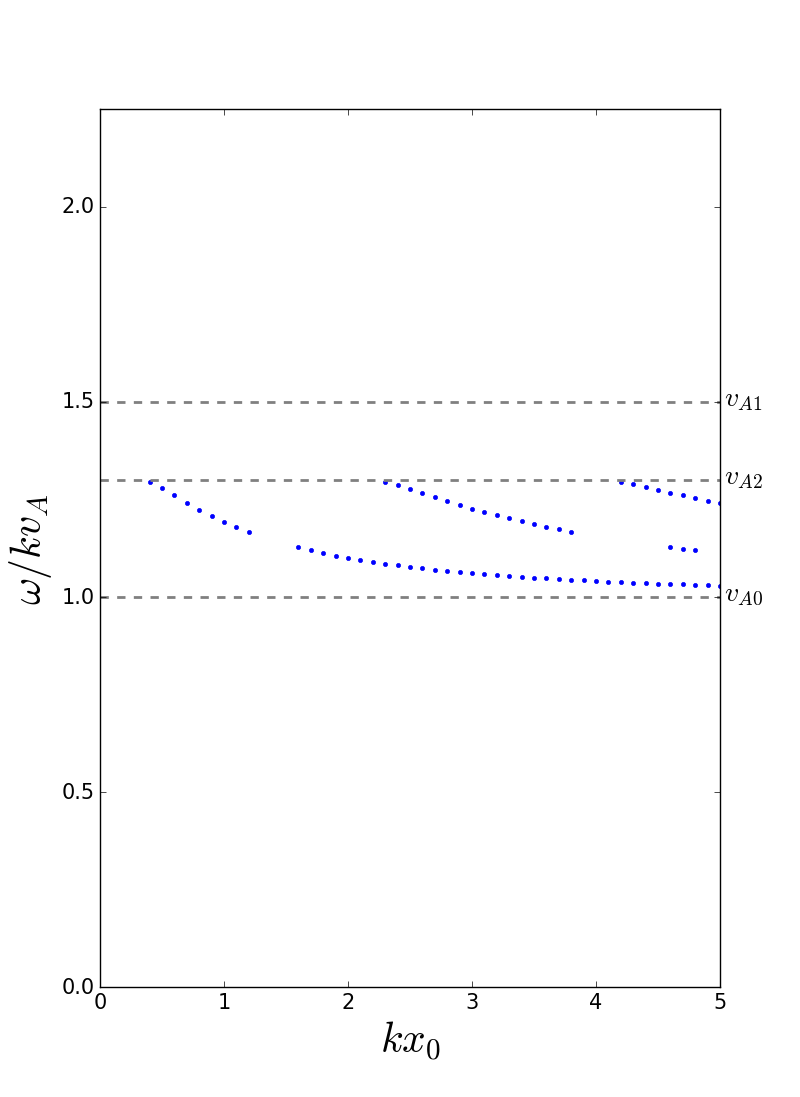
\includegraphics{disp_rel_zero_beta_1.png}}}
		\subfloat[]{\scalebox{0.4}{
				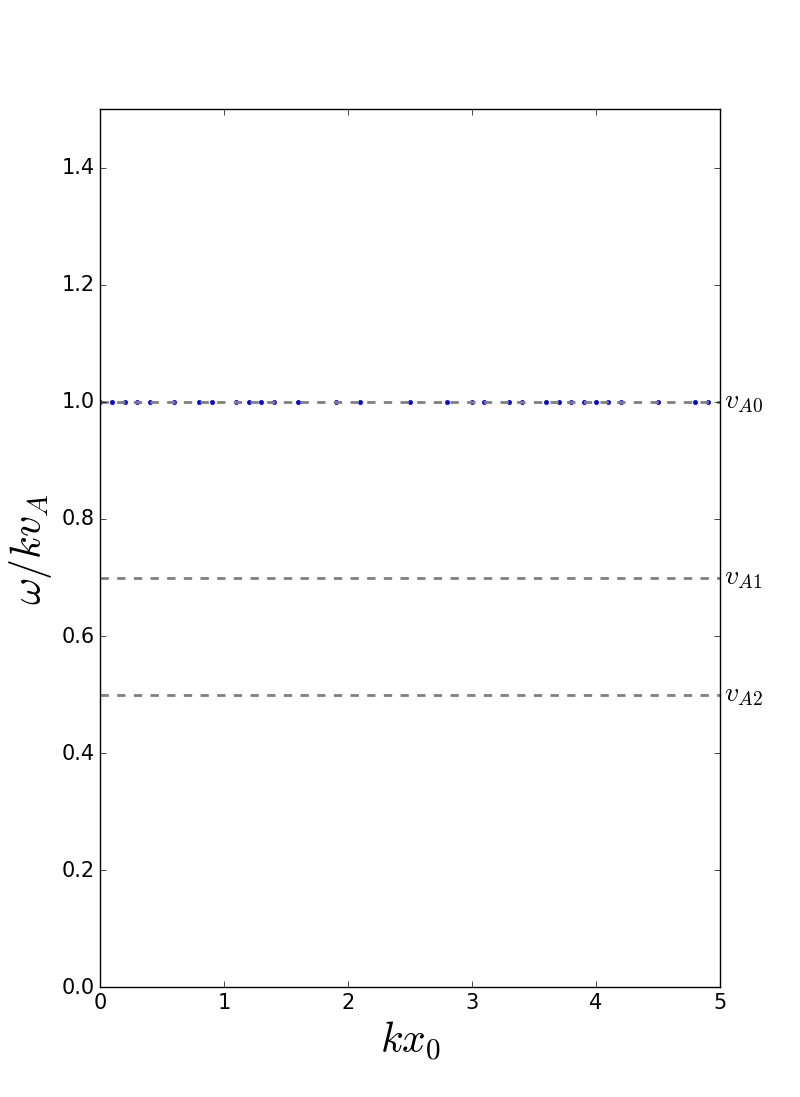
\includegraphics{disp_rel_zero_beta_2.png}}}
	\end{center}
	\caption{Solutions to the zero-beta dispersion relation in two different ordering of the characteristic speeds.}
	\label{fig: zero beta}
\end{figure}


















\acknowledgments
M. Allcock acknowledges the support from the University Prize Scholarship at the University of Sheffield. R. Erd\'{e}lyi acknowledges the support from the UK Science and Technology Facilities Council (STFC) and the Royal Society. 

% inlude mayavi visualisations and link to the website?
\software{Mayavi}

\appendix

\section{Non-standard Laplace transform}\label{app: laplace trans}
Consider a function $f(t)$, whose standard Laplace transform, $F_1(\omega)$, and non-standard Laplace transform, $F_2(\omega)$, are
\begin{equation}
F_1(\omega) = \int_0^\infty f(t) e^{-\omega t} dt,
\quad \text{and} \quad
F_2(\omega) = \int_0^\infty f(t) e^{i\omega t} dt.
\end{equation}
Trivially, $F_1(-i\omega) = F_2(\omega)$. Using the standard inverse Laplace transform, and letting $\gamma$ be real and greater than the real part of all the singularities of $F_1(\omega)$, the original function $f(t)$ can be written
\begin{align}
f(t) & = \frac{1}{2\pi i} \lim_{T\to\infty} \int_{\gamma - iT}^{\gamma + iT} F_1(\omega)e^{\omega t} d\omega, \\
& = \frac{1}{2\pi i} \lim_{T\to\infty} \int_{i\gamma - T}^{i\gamma + T} F_1(-i\omega)e^{-i\omega t} (-id\omega), \\
& = \frac{1}{2\pi} \lim_{T\to\infty} \int_{i\gamma - T}^{i\gamma + T} F_2(\omega)e^{-i\omega t} d\omega.
\end{align}
Therefore, the inverse transform of the non-standard Laplace transform is
\begin{equation}
f(t) = \frac{1}{2\pi} \lim_{T\to\infty} \int_{i\gamma - T}^{i\gamma + T} F_2(\omega)e^{-i\omega t} d\omega.
\end{equation}



%% The reference list follows the main body and any appendices.
%% Use LaTeX's thebibliography environment to mark up your reference list.
%% Note \begin{thebibliography} is followed by an empty set of
%% curly braces.  If you forget this, LaTeX will generate the error
%% "Perhaps a missing \item?".
%%
%% thebibliography produces citations in the text using \bibitem-\cite
%% cross-referencing. Each reference is preceded by a
%% \bibitem command that defines in curly braces the KEY that corresponds
%% to the KEY in the \cite commands (see the first section above).
%% Make sure that you provide a unique KEY for every \bibitem or else the
%% paper will not LaTeX. The square brackets should contain
%% the citation text that LaTeX will insert in
%% place of the \cite commands.

%% We have used macros to produce journal name abbreviations.
%% \aastex provides a number of these for the more frequently-cited journals.
%% See the Author Guide for a list of them.

%% Note that the style of the \bibitem labels (in []) is slightly
%% different from previous examples.  The natbib system solves a host
%% of citation expression problems, but it is necessary to clearly
%% delimit the year from the author name used in the citation.
%% See the natbib documentation for more details and options.

%\begin{thebibliography}{}
%
%\bibitem[Astropy Collaboration et al.(2013)]{2013A&A...558A..33A} Astropy Collaboration, Robitaille, T.~P., Tollerud, E.~J., et al.\ 2013, \aap, 558, A33 
%\bibitem[Bertin \& Arnouts(1996)]{1996A&AS..117..393B} Bertin, E., \& Arnouts, S.\ 1996, \aaps, 117, 393 
%\bibitem[Corrales(2015)]{2015ApJ...805...23C} Corrales, L.\ 2015, \apj, 805, 23
%\bibitem[Ferland et al.(2013)]{2013RMxAA..49..137F} Ferland, G.~J., Porter, R.~L., van Hoof, P.~A.~M., et al.\ 2013, \rmxaa, 49, 137
%\bibitem[Hanisch \& Biemesderfer(1989)]{1989BAAS...21..780H} Hanisch, R.~J., \& Biemesderfer, C.~D.\ 1989, \baas, 21, 780 
%\bibitem[Lamport(1994)]{lamport94} Lamport, L. 1994, LaTeX: A Document Preparation System, 2nd Edition (Boston, Addison-Wesley Professional)
%\bibitem[Schwarz et al.(2011)]{2011ApJS..197...31S} Schwarz, G.~J., Ness, J.-U., Osborne, J.~P., et al.\ 2011, \apjs, 197, 31  
%\bibitem[Vogt et al.(2014)]{2014ApJ...793..127V} Vogt, F.~P.~A., Dopita, M.~A., Kewley, L.~J., et al.\ 2014, \apj, 793, 127  
%
%\end{thebibliography}

\bibliography{Bibliography}

%% This command is needed to show the entire author+affilation list when
%% the collaboration and author truncation commands are used.  It has to
%% go at the end of the manuscript.
%\allauthors

%% Include this line if you are using the \added, \replaced, \deleted
%% commands to see a summary list of all changes at the end of the article.
%\listofchanges

\end{document}

% End of file `sample61.tex'.
